\documentclass[prl,aps,twocolumn, reprint, amsmath,amssymb,showpacs,superscriptaddress]{revtex4}

\usepackage{graphicx}% Include figure files
\usepackage{dcolumn}% Align table columns on decimal point
\usepackage{bm}
\usepackage{graphicx}
\usepackage{epsfig}
\usepackage{epsf}
\usepackage{amssymb}
\usepackage{amsmath}
\usepackage{amsthm}
\usepackage{multirow}
\usepackage{cases}
\usepackage[colorlinks=true,linkcolor=blue,citecolor=blue,pdfauthor={ },pdftitle={ },pdfsubject={ },pdfkeywords={ }]{hyperref}



\newtheorem*{theorem}{Theorem}
\newtheorem*{proposition}{Proposition}


\begin{document}


%\title{Purity Bound Analysis: Application to Open System State Preparation with Coherent Control}
\title{Purity Bounds in Coherently Controlled Open Quantum Systems: Application to Quantum State Engineering}


\author{Jun Li}
\affiliation{Hefei National Laboratory for Physical Sciences at Microscale and Department of Modern Physics, University of Science and Technology of China, Hefei, Anhui 230026, China}

\author{Dawei Lu}
\affiliation{Institute for Quantum Computing and Department of Physics and Astronomy, University of Waterloo, Waterloo, Ontario N2L 3G1, Canada}

\author{Zhihuang Luo}
\affiliation{Hefei National Laboratory for Physical Sciences at Microscale and Department of Modern Physics, University of Science and Technology of China, Hefei, Anhui 230026, China}

\author{Raymond Laflamme}
\affiliation{Institute for Quantum Computing and Department of Physics and Astronomy, University of Waterloo, Waterloo, Ontario N2L 3G1, Canada}
\affiliation{Perimeter Institute for Theoretical Physics, Waterloo, Ontario N2L 2Y5, Canada}
\affiliation{Canadian Institute for Advanced Research, Toronto, Ontario M5G 1Z8, Canada}

\author{Xinhua Peng}
\email{xhpeng@ustc.edu.cn}
\affiliation{Hefei National Laboratory for Physical Sciences at Microscale and Department of Modern Physics, University of Science and Technology of China, Hefei, Anhui 230026, China}
\affiliation{Synergetic Innovation Center of Quantum Information $\&$ Quantum Physics,
University of Science and Technology of China, Hefei, Anhui 230026, China}

\author{Jiangfeng Du}
\email{djf@ustc.edu.cn}
\affiliation{Hefei National Laboratory for Physical Sciences at Microscale and Department of Modern Physics, University of Science and Technology of China, Hefei, Anhui 230026,  China}
\affiliation{Synergetic Innovation Center of Quantum Information $\&$ Quantum Physics,
University of Science and Technology of China, Hefei, Anhui 230026, China}



\begin{abstract}
Precisely characterizing and controlling realistic open quantum systems is one of the most exciting frontiers in quantum sciences and technologies. In this Letter, we derive upper bounds of achievable purity for coherently controlled open quantum systems, which is very useful for assessing dynamics performances. We apply this to a two-qubit nuclear magnetic resonance spin system and implement some tasks of quantum control in open systems at a near optimal performance in view of purity: e.g., increasing polarization and preparing pseudo-pure states. Our work shows interesting and promising applications of environment-assisted quantum dynamics.
\end{abstract}


\pacs{03.67.Lx,76.60.-k,03.65.Yz}

\maketitle

In recent years there have been immense advances in active and precise manipulation of a broad variety of quantum systems. The subject of quantum system control has been developed into a rapidly growing area \cite{DP}, attracting substantial interests from the quantum information science community. One of the fundamental tasks is to design reliable control techniques for quantum systems that are exposed to a dissipative environment \cite{KKSS}.
As dissipation tends to irreversibly affect the system dynamics, it is recognized as one dominant source for information loss and hence must be suppressed.
However, recently it was realized that open system engineering may exhibit surprising advantages in some important aspects \cite{RMBL, Entanglement, SW}. For example, it was shown that the purification efficiency of heat-bath algorithmic cooling protocol can surpass the closed system limit \cite{RMBL}. In other researches \cite{Entanglement}, there emerged great interests in environment-assisted entangled state engineering. Dissipative production of entangled steady states has already been realized
in various experimental setups such as trapped ions \cite{Lin}, superconducting circuit \cite{RTJS} and double quantum dots \cite{SKVCG}.


Although some ideas borrowed from classical control theory (e.g., time optimal control) have been successfully extended to construct methods for steering closed quantum systems \cite{RKGD}, it turns out to be more challenging to follow the same spirit for open quantum systems.
The major reason  comes from the fact proved in \cite{A} that, for a finite dimensional Markovian quantum system, coherent control means cannot fully compensate the irreversibility of the dynamics. In fact, to what extent can the evolving tendency of the system be changed depends not only on the external operations but also the structure of the relaxation mechanisms. This certainly increases difficulties in understanding the controllable properties of the system, which thus hinders the devising of general control methodology.
Previous research has shown that one can characterize the reachable set on the states of a single qubit both qualitatively \cite{A} and quantitatively \cite{Y, RBR}.
However, it is difficult to generalize these results to higher dimensional quantum systems \cite{R}.

An alternative approach to the problem is to explore the dynamical behaviors of purity function of the system. Purity, as an important concept quantifying the incoherent impacts from the environment, is particularly suited for studying how relaxation noises impose the restrictions on the achievable region of states. For example, one basic result for \emph{unital} systems (where the equilibrium state is the maximally mixed state) states that the purity function must be monotonically decreasing with time regardless of the controls \cite{LSA}. For the case of \emph{non-unital} dynamics, the situation is more complicated, since purification can occur depending on applied control protocols. It is thus natural to consider that, given a realistic open quantum system, what is the upper bound of purity that a system can reach. The determination of bounds on quantum dynamics is relevant in several
disciplines of chemistry and physics. In this Letter, we derive the maximally achievable  purity of coherently controlled relaxing systems under certain relaxation model. To this end, we study the evolution of purity function under appropriate assumptions of system's relaxation mechanisms. Moreover, our ideas are experimentally implemented using nuclear magnetic resonance (NMR) techniques.


\emph{Problem setting} -- Consider a controlled $n$-qubit open system governed by the Lindblad equation \cite{Lindblad}
\begin{equation}
\label{Lindblad}
\dot \rho   =  - i[H,\rho ] +  \mathcal{R}\rho ,
\end{equation}
where $H$ incorporates both system Hamiltonian $H_0$ and external control Hamiltonian $H_{ext}$, and $\mathcal{R}$ is the relaxation superoperator of Lindblad type:
\begin{equation}
\mathcal{R}\rho =  \sum\limits_\alpha  {{\gamma _\alpha }\left( {2{L_\alpha }\rho L_\alpha ^\dag  - L_\alpha ^\dag {L_\alpha }\rho  - \rho L_\alpha ^\dag {L_\alpha }} \right)} ,
\end{equation}
where ${{L_\alpha }}$ are called Lindblad operators representing the coupling with the environment, and $\gamma_\alpha$ are positive relaxation rates.

Let $\mathcal{B} = \left\{ B_s \right\}$ is a complete set of normalized base operators \cite{K, SW}, consisting of $4^{n}$ product operators ${{ B}_s} = \frac{1}{2^{n/2}} \prod\limits_{k = 1}^n { \sigma _{i}^k}, (0 \le s \le {4^n} - 1)$, where $k$ is an index for the spin and $i \in \left\{ {0,1,2,3} \right\}$, corresponding to the unit operator and Pauli operators ($\left\{ { I,{{ \sigma }_x},{{ \sigma }_y},{{ \sigma }_z}} \right\}$). Here $Tr({{ B}_s}{{ B}_r}) = {\delta _{sr}}$. The $n$-qubit state $\rho$ can be  expressed as: $\rho = {I^{ \otimes n}}/{2^n} + \sum\nolimits_{s = 1}^{{4^n-1}} {{\bm{r}_s}{B_s}} $ (${\bm{r}_s} = \text{Tr}\left( {\rho {B_s}} \right)$).
Hence Eq. \eqref{Lindblad} is transformed into a real $4^n -1$ dimensional inhomogeneous vector differential equation:
\begin{equation}
\label{Bloch}
\bm{\dot  r} = \mathbf{H} \bm{r} -  \mathbf{R} ( \bm{r} - {\bm{r}_{eq}}),
\end{equation}
where $\mathbf{H}$, $\mathbf{R}$  and $\bm{r}_{eq}$ are $4^n-1$ dimensional matrices with the entries ${\mathbf{H}_{kj}}  = \text{Tr} \left( {-i{B_k}\left[H, {{B_j}} \right]} \right)$, ${\mathbf{R}_{kj}} = \text{Tr}\left(- {{B_k}\mathcal{R}{B_j}} \right)$ and $\bm{r}_{eq,k}  = \sum\nolimits_j {{\mathbf{R}}_{kj}^{ - 1}{\text{Tr}}\left( {{B_j}{\mathcal R}{I^{ \otimes n}}} \right)/{2^n}} $, respectively. Here $\mathbf{H}$ is antisymmetric and $\mathbf{R}$ (relaxation matrix) is symmetric positive semidefinite.

In order to further simplify this problem, we project the system dynamics into the diagonal subspace through diagonalization procedure \cite{Y, RBR}. Let $\rho = U \Lambda U^\dag$ with a diagonal matrix $\Lambda$ and a unitary matrix $U \in SU(2^n)$. In the vector representation $\mathcal{B}$, the diagonalization procedure can be written as $\bm{r} = \mathbf{U} \bm{x}$, where $\bm{x}$ ($ \in \mathbb{R}^{2^n -1}$) is the representation of $\Lambda$ and $\mathbf{U}$ is that of $U$, with respect to basis $\mathcal{B}$. For convenience, we choose a specific order to the diagonal elements ${\left\{ {{\Lambda _{kk}}} \right\}_{k = 1}^{2^n}}$, which induces an order to the coordinates $\left\{ 0 \right\} \cup {\left\{ {{\bm{x}_k}} \right\}_{k = 1}^{2^{n }- 1}}$. The chosen order thus uniquely determines a \emph{representative region} $\Sigma \subset \mathbb{R}^{2^n -1}$, in which each point is a \emph{representative point} of its unitary orbit and two points are unitarily equivalent only if they coincide.
Consequently, any evolution of the system can be projected into a continuous trajectory in the region $\Sigma$. Substituting the diagonalization procedure, Eq. (\ref{Bloch}) is reduced into a $2^n -1$ dimensional dynamical equation \cite{Y}
\begin{equation}
\label{Projection}
\bm{\dot x} = - {\left[ {{\mathbf{U}^T}\mathbf{R}\mathbf{U}} \right]_\mathbf{p}}(\bm{x} - \left[ {\mathbf{U}^T}{\bm{x}_{eq}}\right]_\mathbf{p}),
\end{equation}
where $\bm{x}_{eq}$ is the representative point of $\rho_{eq}$ in $\Sigma$, ${\mathbf{U}^T}$ is the transpose of ${\mathbf{U}}$, and $[\cdot]_\mathbf{p}$ denotes the diagonal subspace part of its argument.
The vector forms of Lindblad equation, i.e., Eqs. (\ref{Bloch}) and (\ref{Projection}), can make the dynamics analysis more convenient.

Our goal is to determine the purity bounds for realistic open physical systems and use the bounds to characterize the transfer efficiency bound between two interconvertible directions in $\Sigma$. Clearly the problem here extends the concept of \emph{universal bound on spin dynamics} \cite{SSGGNS} (bounds on the regions of operators in Liouville space being interconvertible by unitary transformations) to the case of unitary and non-unitary transformations in open systems.
The subsequent analysis is based on some assumptions about the considered open quantum system: $(i)$ the system is relaxing, namely there exists a unique equilibrium state $\rho_{eq}$ \cite{RH}; $(ii)$ $\rho_{eq}$ is diagonal in the eigenbasis of system Hamiltonian $H_0$;  $(iii)$ the relaxation matrix $\mathbf{R}$ in the basis $\mathcal{B}$ admits the direct sum decomposition (\emph{secular approximation}) \cite{KM}: $\mathbf{R} = \mathbf{R_p} \oplus \mathbf{R_c}$, where $\mathbf{R_p}$ and $\mathbf{R_c}$ represent the relaxation matrices in the population and coherence subspace, respectively; $(iv)$ longitudinal relaxation rates $\lambda (\mathbf{R_p})$ are slower than transversal relaxation rates $\lambda (\mathbf{R_c})$: ${\lambda _{\max }}({\mathbf{R}_\mathbf{p}}) \le {\lambda _{\min }}({\mathbf{R}_\mathbf{c}})$; $(v)$ any coherent unitary control can be implemented before relaxation effects become important. These assumptions are valid in many practical physical systems, e.g., spin-based systems.


\emph{Maximally accessible purity}---
Recalling the definition of the purity $p=\text{Tr}(\rho^2)$, then $p=1/2^n + {\bm{r}^T} \bm{r}$ in the vector representation $\mathcal{B}$.
The time-evolution of the purity can thus be expressed as
\begin{equation}
\dot p  = d ({\bm{r}^T} \bm{r}) /dt  =  - 2{\bm{r}^T} \mathbf{R} (\bm{r} - {\bm{r}_{eq}}).
\end{equation}
The set of states satisfying $\dot p = 0$ determines an ellipsoid in $\mathbb{R}^{4^n-1}$, which depends only upon $\mathbf{R}$ and $\bm{r}_{eq}$. Due to positive definiteness of $\mathbf{R}$, for any state $\bm{r}$ outside the ellipsoid there must be $\dot p (\bm{r}) < 0$. Let $S$ denote the smallest sphere enclosing the ellipsoid. Then we have that: $(i)$ the equilibrium state $\bm{r}_{eq}$ is located inside $S$, and $(ii)$ the evolution direction of any state $\bm{r}$ on $S$ is towards the inner side of $S$. Thus starting from $\bm{r}_{eq}$, the system can not be driven outside $S$ by coherent controls. Therefore, we can obtain an upper bound on the purity $p$ by solving the following optimization problem:
\begin{numcases}{}
\label{Optimization}
\max & $p (\bm{r})= 1/2^n + {\bm{r}^T} \bm{r}$,  \nonumber \\
\text{s.t.} & $\dot p (\bm{r}) =  - 2{\bm{r}^T} \mathbf{R} (\bm{r} - {\bm{r}_{eq}}) =0.$
\end{numcases}
This problem can be seen as an instance of \emph{quadratic programming over an ellipsoid constraint}, which is easy in the sense of computational complexity and can be solved with well-developed algorithms \cite{FP}. Furthermore, to find a way approaching the maximum purity, we need \cite{S1}:

\begin{proposition}
Let $\mathcal{P}_{2^n}$ denotes the collection of $2^n!$ permutation operations on diagonal elements of the density matrix. Let $\mathcal{Q}_{2^n}$ be the corresponding set of $\mathcal{P}_{2^n}$ in $\mathcal{B}$. Suppose that the relaxation matrix $\mathbf{R}$ satisfies $\mathbf{R} =  \mathbf{R_p} \oplus \mathbf{R_c}$ and ${\lambda _{\max }}({\mathbf{R_p}}) \le {\lambda _{\min }}({\mathbf{R_c}})$ (i.e., the assumptions $(iii)$ and $(iv)$ mentioned above), then there exists an element $\mathbf{Q} \in \mathcal{Q}_{2^n}$ so that
\begin{equation}
\label{prop1}
\dot p(\bm{r})  \le  - 2{(\mathbf{Q}{\bm{x}})^T}\mathbf{R}(\mathbf{Q}{\bm{x}} - {\bm{x}_{eq}}) \equiv \dot p(\mathbf{Q}\bm{x})  .
\end{equation}
\end{proposition}

Accordingly, for a state $\bm{r} = \mathbf{U} \bm{x} $ at some instant $ t_0$, if there exists an element $\mathbf{Q} \in \mathcal{Q}_{2^n}$ to make $\dot p(\mathbf{Q}\bm{x}) > 0$, it is possible to increase the purity from the state $\bm{r}$ at $t_0 + dt$. This proposition also tells us the maximum of $\dot p(\bm{r})$.
Therefore, one can asymptotically approach the maximally accessible purity of state through repeatedly applying the following three steps: $(i)$ finding out an element $\mathbf{Q} \in \mathcal{Q}_{2^n}$ that maximizes $\dot p(\bm{r}) $ at a current state $\bm{r}$; $(ii)$ transforming the state $\bm{r}$ into the diagonal state $\mathbf{Q} \bm{x}$ by coherent controls $\mathbf{U}$ and $\mathbf{Q}$; $(iii)$ performing free evolution with a small duration $dt$ to update the current state $\bm{r}$.  Repeating applying the procedure till there does not exist any $\mathbf{Q} \in \mathcal{Q}_{2^n}$ to make $ \dot p(\mathbf{Q}\bm{x}) > 0$, i.e., $\dot p(\mathbf{Q}\bm{x}) \le 0 $ for all the $2^n!$ elements $\mathbf{Q} \in \mathcal{Q}_{2^n}$, which implies the purity at the current state $\bm{r}$ is an extremum. Note that any extremum found here should be the maximum, since the purity is a convex function.

In order to make the control protocol experimentally more feasible, we focus on such periodically modulated systems as ${\left[{\tau } - {V} \right]_m}$. Here $V$, $\tau$ and $m$ denote a unitary operation, free evolution time and the number of cycles, respectively. Provided the assumption $(v)$ on the open system (i.e., the time to implement $V$ can be ignored),  we can then be free to assume that each of $V$ runs over the entire group $SU(2^n)$. Note that a generic periodic control sequence is ${\left[ {\tau _M} - {{V_M} - \cdots -{\tau _1}} - {V_1} \right]_m}$. Its theoretical analysis and experimental realization are not easier than the general sequence $ [ {\tau _M} - {{V_M} - \cdots -{\tau _1}} - {V_1} ]$. In open systems, periodic control promises the capability of  driving the system asymptotically to some periodic steady state. This is due to that a controlled relaxing system leads to a strictly contractive quantum channel, i.e., the distance of any fixed pair of initial states is a strictly decreasing function with the time \cite{RH}. Such a property makes it possible to periodically retain a desired state. The desired state can be the fixed point of the controlled dynamics.

Suppose a periodic control sequence ${\left[{\tau } - {V} \right]_m}$ results in a periodically steady state $\rho_{ss}$, which is mathematically written as: $\mathcal{E}_{\tau} \circ \mathcal{E}_{V} \rho_{ss} = \rho_{ss}$ (here $\mathcal{E}_{V}$ and $\mathcal{E}_{\tau}$ are the associated dynamical maps, related to the operation $V$ and the evolution $\tau$ \cite{RH}), respectively. Then for any state unitarily equivalent to $\rho_{ss}$, say $\mathcal{E}_{W} \rho_{ss}$ ($W \in SU(2^n)$), there exists an associated periodic preparation sequence ${\left[ W -  {\tau} - {V} - W^\dag \right]_m}$ so that $\mathcal{E}_{W} \rho_{ss}$ will be its fixed point. Without the loss of generality, we only discuss the case of preparing diagonal states. Then we can prove \cite{S1}
\begin{proposition}
Each element $\mathbf{Q}_k$ ($k=1,...,2^n!$) in $\mathcal{Q}_{2^n}$ is associated with two definite quadratic forms
\begin{align}
& E_k =  - 2{(\mathbf{Q}_k {\bm{x}})^T} \mathbf{R} (\mathbf{Q}_k {\bm{x}} - {\bm{x}_{eq}}),  \nonumber \\
& F_k = 4 {(\mathbf{Q}_k{\bm{x}} - {\bm{x}_{eq}}/2)^T} \mathbf{R}^2 (\mathbf{Q}_k{\bm{x}} - {\bm{x}_{eq}}).
\end{align}
Because of permutation symmetry, there exists a constant $C$ such that for each $k$, $E_k = C$ is the smallest ellipsoid enclosing $F_k = 0$.
Then in the representative region $\Sigma$,  it is impossible to steer the system from $\bm{x}_{eq}$ to any state that locates outside the ellipsoid
\begin{equation}
E: - 2{{\bm{x}}^T} \mathbf{R} ( {\bm{x}} - {\bm{x}_{eq}}) = C,
\end{equation}
through the periodic control sequences ${\left[ {\tau } - {V}  \right]_m}$.
\end{proposition}
Hence, according to this proposition, the purity of this system driven by ${\left[{\tau } - {V} \right]_m}$ can not surpass the smallest sphere enclosing the ellipsoid $E=C$ (i.e., \emph{the purity bound by the periodic sequence ${\left[{\tau } - {V} \right]_m}$}).

\emph{Applications on two-qubit system}.---
We used the $^{13}C$-labeled chloroform dissolved in $d_6$-acetone as a two-qubit system to test the applicability of open system control method. Our experiments were carried out on a Bruker Avance \uppercase\expandafter{\romannumeral3} 400 MHz ($B_0$ = 9.4 T) spectrometer at room temperature. The operator basis $\mathcal{B}$ for the two-qubit system is
\begin{align}
\mathcal{B}_2 = & \{ II,ZI,IZ,ZZ,XI,YI,XZ,YZ,   \nonumber \\
& IX,IY,ZX,ZY,XY,YX,XX,YY \} /2,   \nonumber
\end{align}
where $X := \sigma_x$, $Y : = \sigma_y$ and $Z : = \sigma_z$. The natural Hamiltonian reads: $H_S = \pi ( - \gamma_\text{C} B_0 ZI -  \gamma_\text{H} B_0 IZ+ J/2 ZZ)$,
where $\gamma_\text{C}$ and $\gamma_\text{H}$ are the gyromagnetic ratios of nuclei $^{13}$C and $^{1}$H, respectively, and $J = 214.5$Hz is the scalar coupling constant.
The equilibrium state at the room temperature is $\rho_{eq} \approx II/4 + \epsilon_C ZI + \epsilon_H IZ$ with the polarization $ \epsilon_C \approx \epsilon_H/4  \equiv  \epsilon  \sim 10 ^{-5}$.
In the double rotating frame, the system relaxation matrix $\mathbf{R}$ would take a kite-like appearance under secular approximation \cite{KM}.
%The underlying principle is that, the system energy level differences are much larger than the relaxation rates, so in the interaction picture, the cross relaxation parameters between the population subspace and the coherence subspace are added with fast oscillating phases. This effectively decoupled the population subspace relaxation from the coherence subspace relaxation.
The simplified structure dramatically reduces the complexity of experimentally estimating the effective relaxation parameters. We measured $\mathbf{R}$ \cite{S2} and found that the longitudinal relaxation rates are almost an order of magnitude slower than the transversal relaxation rates.

\begin{figure*}
\centering
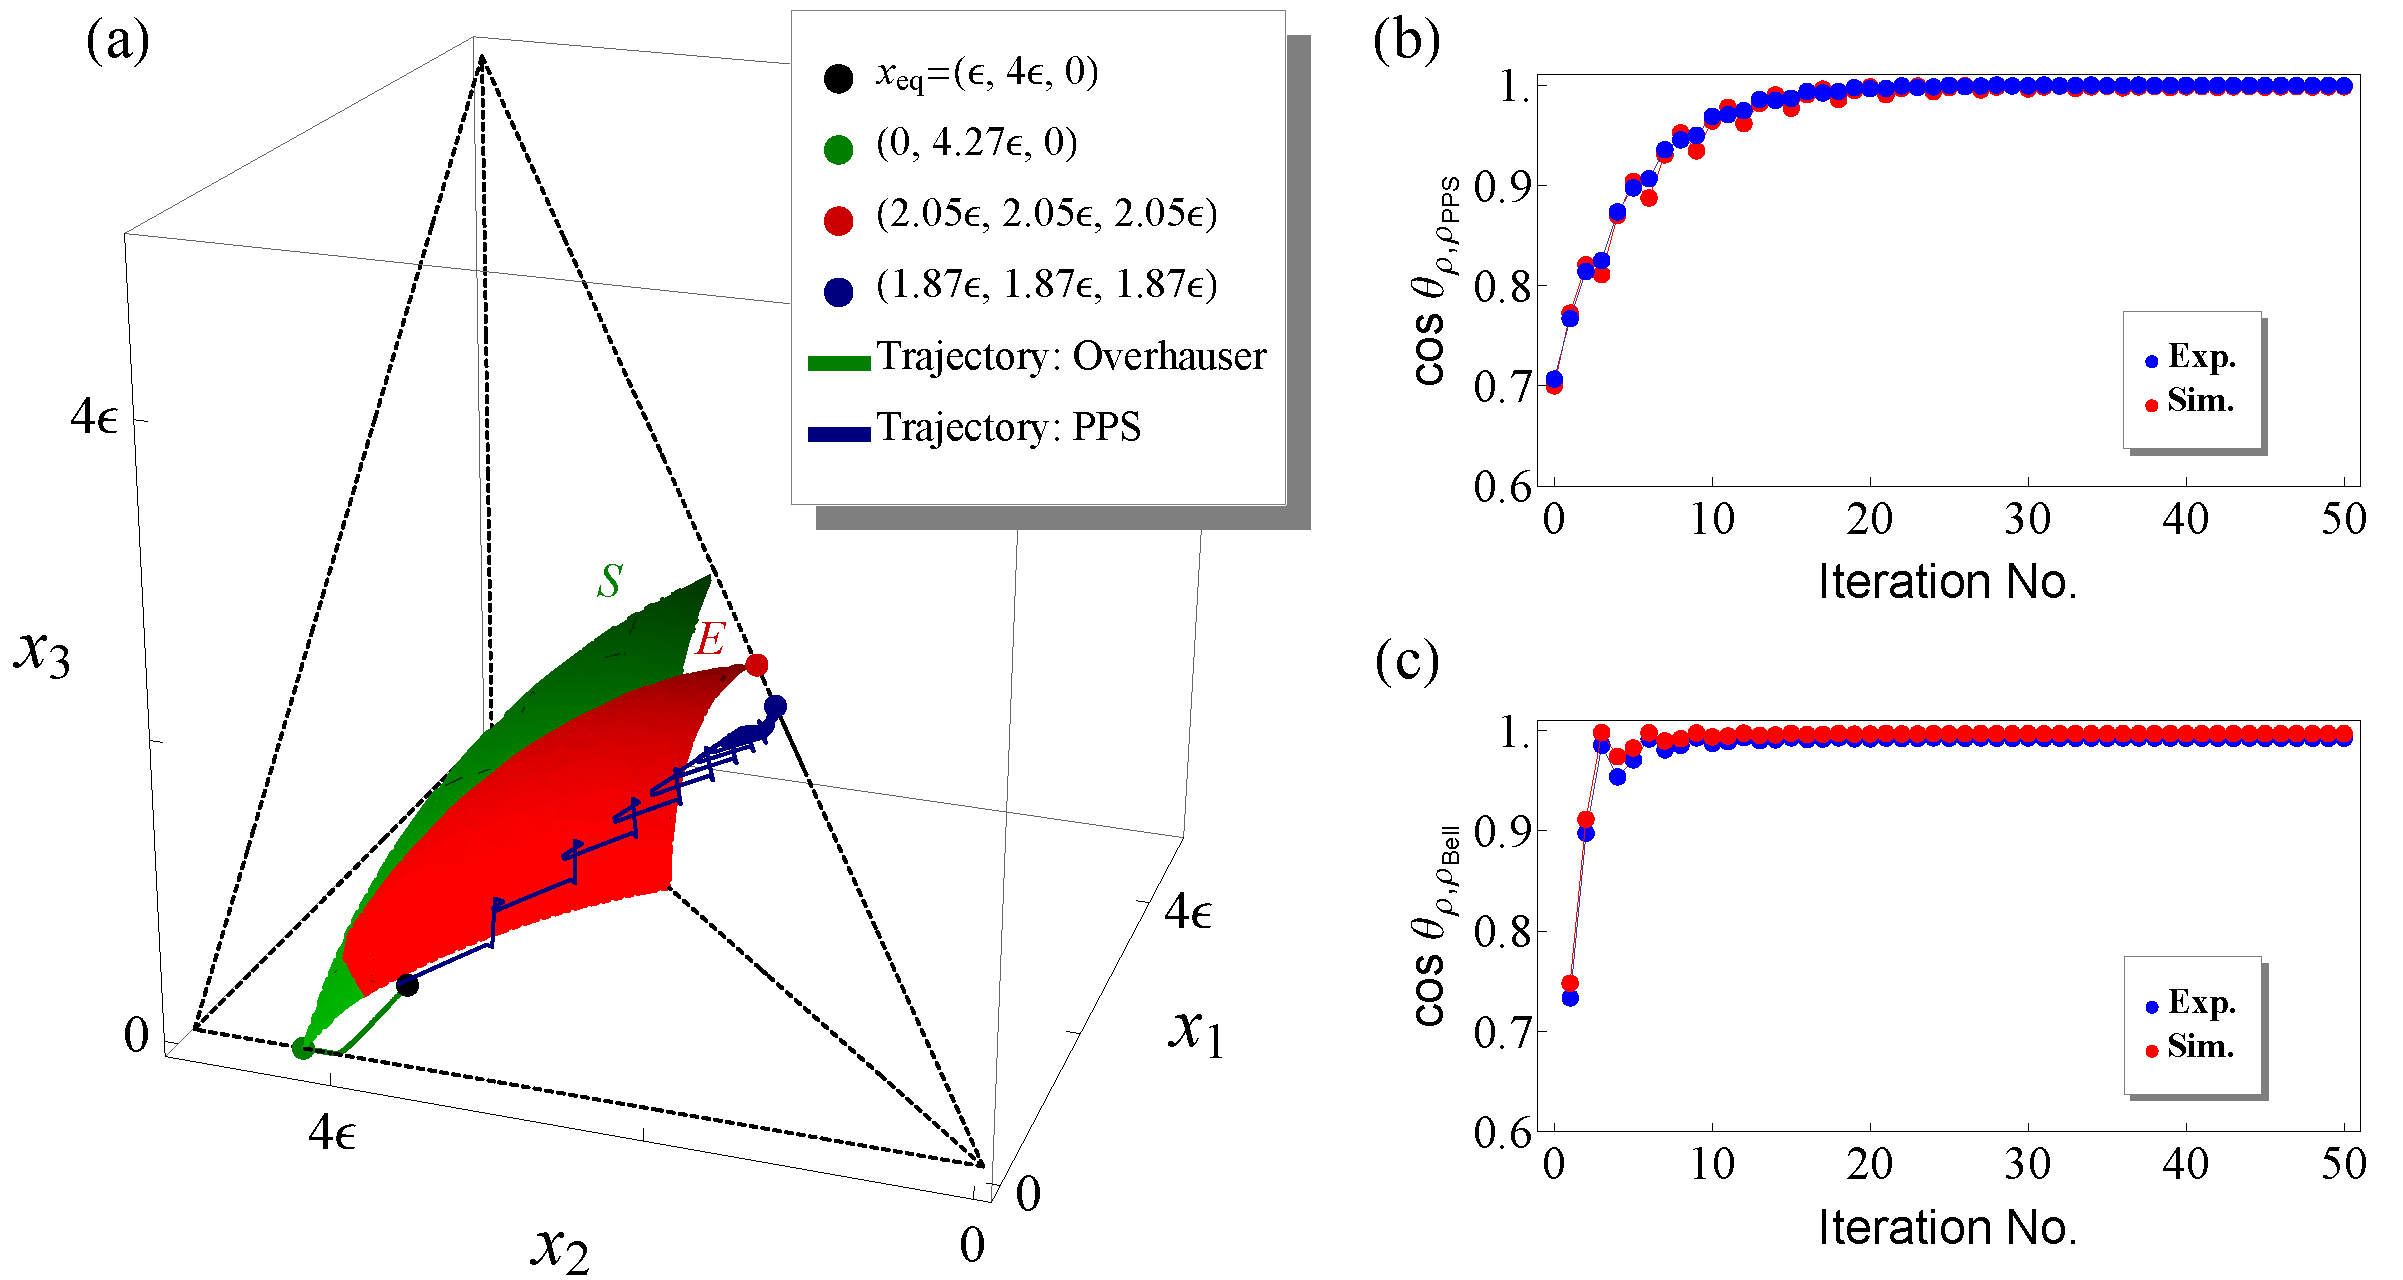
\includegraphics[width=0.75\linewidth]{Figures/Figure}
%\caption{(a) Illustrations of the results on our chloroform system, including: (i) representative region $\Sigma: 0 \le x_3 \le x_1 \le x_2$; (ii) sphere (green) $S: \bm{x}^T \bm{x} = 18.06 \epsilon^2$; (iii) ellipsoid (red) $E: - 2{{\bm{x}}^T} \mathbf{R} ( {\bm{x}} - {\bm{x}_{eq}}) = -0.0523 \epsilon ^2$; (iv) projected trajectories (simulation) of nuclear Overhuaser and PPS preparation evolutionary dynamics. (b)-(c) The resulting PPS $\rho_{pps}$ under periodic control $\left[ \tau - \mathbf{V} \right]_m$, in which $\tau = 1.5$s; $\mathbf{V}$ is determined according to Eq. (\ref{V}) and implemented through the sequence ${R_y^{\text{H}}(90^\circ) - 1/(2J) - R_x^{\text{H}}(90^\circ) - R_y^{\text{C}}(90^\circ) - 1/(2J) - R_x^{\text{C}}(90^\circ)}$.  The data clearly display how the system converges to a pseudopure state, and numerical simulation with the master equation Eq. (\ref{Bloch}) agrees well with experimental results. (d) Simulation result: relative error of the prepared PPS due to imperfections of control fields present in the $^{13}$C channel and $^1$H channel. (e) The resulting Bell state $\rho_{Bell}$ under periodic control $\left[ \mathbf{W} - \tau - \mathbf{V} - \mathbf{W}^T \right]_m$, in which $\mathbf{W}$ is determined according to Eq. (\ref{W}).}
\caption{(a) Purity bounds for our two-spin open system in the representative region $\Sigma: 0 \le x_3 \le x_1 \le x_2$: for a general control denoted by the green sphere $S: \bm{x}^T \bm{x} = 18.06 \epsilon^2$, and for the periodic control sequence ${\left[ {\tau } - {V}  \right]_m}$ denoted by the red ellipsoid surface $E: - 2{{\bm{x}}^T} \mathbf{R_p} ( {\bm{x}} - {\bm{x}_{eq}}) = -0.0523 \epsilon ^2$, which are obtained based on the measured relaxation matrix $\mathbf{R}$ \cite{S1}. The simulated projected evolutionary trajectories of NOE (green line) and PPS preparation (blue line). Experimental results (blue data points) for PPS preparation by using periodically steady state method for (b) a diagonal PPS $\rho_{PPS}$ with $\vert \psi \rangle  = \vert 00 \rangle$ and (c) a pseudo-entangled state $\rho_{Bell}$ with $\vert \psi \rangle  = (\vert 00 \rangle + \vert 11 \rangle)/ \sqrt{2}$, along with the simulated results (red data points). Here $\theta_{\rho,\rho_{tar}}  = \arccos \left[ \bm{x}^T \bm{x}_{tar} / \sqrt{ (\bm{x}^T \bm{x})  (\bm{x_{tar}}^T \bm{x_{tar}})}  \right]$ is the angle between the system state $\rho$ and the target-state ($\rho_{tar}$) direction in the vector of coherence representation, with the target state $\rho_{tar} = \rho_{PPS}$ or  $\rho_{Bell}$. }
\label{Figure}
\end{figure*}


According to Eq. (\ref{Projection}), we project the 15-dimensional system dynamics into a 3-dimensional differential equation. The representative region $\Sigma$ is illustrated in Fig. \ref{Figure}(a), where we have chosen the order $0 \le x_3 \le x_1 \le x_2$.
In the region, we derived the sphere $S$ representing the upper bound of the system purity and the ellipsoid $E$ representing a bound surface for the ${\left[ {\tau } - {V}  \right]_m}$ sequence, based on the measured relaxation matrix $\mathbf{R}$.


Our first focus is the intersection between $S$ and the $\bm{x}_2$ axis: $(0, 4.27\epsilon, 0)$, corresponding to the maximal $^{1}$H polarization without $^{13}$C polarization. This state might be approached by the nuclear Overhauser effect (NOE)  \cite{L}. For a heteronuclear two-spin system, the magnetization of one of the spins could be strongly affected (in some cases, even enhanced) by a weak irradiation of the other spin for a sufficiently long time, while the polarization of the irradiated nuclei will be saturated \cite{L}.  In the experiment, we drove the system into a steady state measured as $\bm{x}_{ss} = (0, 4.25\epsilon, 0)$ by a $^{13}$C  irradiation with the magnitude of 1000Hz and the duration of 10s. The $^{1}$H polarization is slightly enhanced and fairly close to the upper bound.

Our purity bound analysis thus leads  to a new view of the NOE experiments. The polarization transfer efficiency in the NOE experiments is nearly optimal, which shows the advantages of environment-assisted quantum control over the closed systems.  Moreover, it generalizes the results of heat-bath algorithmic cooling schemes. According to the purification limits derived in \cite{RMBL}, it is impossible to cool the proton in our system through the ``compression and refresh" iterative procedure. This is due to the different underlying relaxation mechanisms assumed. In heat-bath algorithmic cooling schemes, it is considered that each qubit undergoes their respective $T_1$ and $T_2$ processes. But in NOE, cross-relaxation mechanisms are essential for the $^{1}$H polarization enhancement \cite{L}. Thus the performance can be further improved if more general relaxation mechanisms are taken into account.
%Design or evaluation of experimental schemes for trans- fer of coherence or polarization between states in quantized systems requires a clear understanding of which regions of operators in Liouville space are interconvertible by avail- able propagators. Thi
%Overhauser phenomenon is also interesting from the open-system algorithmic cooling aspect of view.


Next we turn to the application of open system coherent control to quantum state engineering.
We consider creating pseudopure states (PPS) \cite{CPH, GC, KCL} from the equilibrium state, which is  an often used initialization step for NMR quantum computation. The task can not be done merely with unitary operations. Previous methods of PPS preparation  \cite{PPS} involve temporal averaging (by summing different experimental results) or spatial averaging (by applying gradient fields) to realize non-unitary operations.  Relaxation effects in open systems are itself a natural  resource of non-unitary processes.  Utilizing the above method of periodically steady state in open quantum systems, we prepared a PPS by designing a periodic control sequence so that the PPS is the fixed point of the dynamics. Although the current experiments were performed on the two-qubit system as an example, the idea can apply to general cases.

%
%Secondly, relaxation cause severe decoherence effects if PPS preparation takes relatively long time. For example, it's hard to prevent a nontrivial quantum state from relaxing to thermal equilibrium. Both of the two problems call for the study of non-unitary control methods.
A PPS can be written as the form of $\rho_{pps} = (1 - \eta) I^{\otimes n}/2^n + \eta \vert \psi \rangle \langle \psi \vert$, where $\eta$ is the \emph{effective purity}. For a two-qubit system, $\rho_{pps} =  II/4 + \eta/4 (ZI + IZ + ZZ)$ on the basis $\mathcal{B}$ in the representative region $\Sigma$. The direction of ${x}_1 = {x}_2 = {x}_3$ specifies the \emph{PPS direction} and the distance from the origin (0,0,0) specifies the effective purity $\eta$. According to our purity bound analysis above, the intersection between the ellipsoid surface $E$ and the PPS direction limits the possible maximal value for $\eta$ through the periodic control sequence ${\left[ {\tau } - {V}  \right]_m}$.
By a ``coefficient-averaging process", we can make $\rho_{pps}$ is an approximate fixed point of $\left[ \tau - {V} \right]_m$, when $\mathbf{V}$ (the representation of ${V}$ in the basis $\mathcal{B}$) is a cyclic permutation of the coordinates of $\bm{x}$ (e.g., $\mathbf{V}(x_1, x_2, x_3)^T = (x_2, x_3, x_1)^T$), and the dynamical map $\mathcal{E}_{\tau}$ satisfies $|| \mathcal{E}_{\tau} - I || \ll 1$. Depending on our measured $\mathbf{R}$, as long as $\tau < 2.0s$, the periodically steady state will always converge to the PPS direction, except for a different effective purity $\eta$ \cite{S1}. In experiments, we found the maximal effective purity ($\eta \approx 7.48 \epsilon$) when $\tau = 1.5$s, which is higher than $\eta \approx 6.12 \epsilon $ by conventional spatial averaging method \cite{P}. The  gap between this and the bound given by the surface $E$ can be attributed to two reasons: $(i)$ the imperfection on the experimentally measured $\mathbf{R}$; $(ii)$ the assumption of ignoring the relaxation during the operation $\mathbf{V}$ for deriving the bound surface $E$. We also experimentally prepared a periodically steady pseudo-entangled state $\rho_{Bell}$ by the sequence $\left[ W - \tau - V - W^{\dagger} \right]_m$ where a unitary operation
$W$ transforms $\rho_{pps}$ to $\rho_{Bell}$. Figure \ref{Figure}(b) and (c) show the experimental results along with numerical simulations with the Lindblad equation Eq. (\ref{Bloch}), which indicates that the realistic open system can periodically keep in any desired state within the reachable set, including the entangled states.

To conclude, we presented the purity bounds for coherently controlled Markovian systems, which is valuable for assessing open system control schemes and guiding numerical pulse searching algorithms. According to this bound analysis, we further investigated NOE and quantum state engineering experiments in the open system framework. The subtleness of the environment can show the new lights on the capability of controlling quantum systems, especially for those regimes being lack of full controllability \cite{XYS, L}. Future work will concentrate on incorporating the present work with other open system control models, such as reservoir engineering and/or other incoherent means \cite{PR}. Besides, the bounds on quantum dynamics can be applicable in magnetic resonance spectroscopy including bio-medical diagnosis, and other physical and chemical systems.


\section{Acknowledgments}
This work is supported by the National Key Basic Research Program of China (Grant No. 2013CB921800 and No. 2014CB848700), the National
Science Fund for Distinguished Young Scholars Grant No. 11425523, National Natural Science Foundation of China under Grant Nos. 11375167, 11227901, 91021005, the Chinese Academy of Sciences, the Strategic Priority Research Program (B) of the CAS (Grant No. XDB01030400).












\begin{thebibliography}{28}
\bibitem{DP} D. Dong and I. R. Petersen, IET Control Theory Appl. \textbf{4}, 2651 (2010).

\bibitem{KKSS} N. Khaneja \emph{et al}, J. Magn. Reson. \textbf{162}, 311 (2003); N. Khaneja \emph{et al}, J. Magn. Reson. \textbf{172}, 296 (2005); B. Bonnard and D. Sugny, SIAM J. Control Optim. \textbf{48}, 1289 (2009); M. Lapert, Y. Zhang, M. Braun, S. J. Glaser, and D. Sugny, Phys. Rev. Lett. \textbf{104}, 083001 (2010).

\bibitem{RMBL} L. J. Schulman, Tal Mor, and Y. Weinstein, Phys. Rev. Lett. \textbf{94}, 120501 (2005); C. A. Ryan, O. Moussa, J. Baugh, and R. Laflamme, Phys. Rev. Lett. \textbf{100}, 140501 (2008).

\bibitem{SW} S. G. Schirmer and X. Wang, Phys. Rev. A \textbf{81}, 062306 (2010).

\bibitem{Entanglement} S. Diehl \emph{et al}, Nature Phys. \textbf{4}, 878 (2008); F. Verstraete, M. M. Wolf and J. I. Cirac, Nature Phys. \textbf{5}, 633 (2009); A. Pechen, Phys. Rev. A \textbf{84}, 042106 (2011); F. Ticozzi and L. Viola, Quantum Inform. Compu. \textbf{14}, 0265 (2014).

\bibitem{Lin} Y. Lin \emph{et al}, Nature (London) \textbf{504}, 415 (2013).

\bibitem{RTJS} F. Reiter, L. Tornberg, G. Johansson, and A. S. S{\o}rensen Phys. Rev. A \textbf{88}, 032317 (2013).

\bibitem{SKVCG} M. J. A. Schuetz, E. M. Kessler, L. M. K. Vandersypen, J. I. Cirac and G. Giedke, Phys. Rev. Lett. \textbf{111}, 246802 (2013).



\bibitem{RKGD} S. Shi and H. Rabitz, Chem. Phys. \textbf{139}, 185 (1989); A. P. Peirce, M.A. Dahleh, and H. Rabitz, Phys. Rev. A \textbf{37}, 4950 (1988); N. Khaneja, R. W. Brockett, and S. J. Glaser, Phys. Rev. A \textbf{63}, 032308 (2001); N. Khanejaa, T. Reissb, C. Kehletb, T. Schulte-Herbr{\"{u}}ggen, and S. J. Glaser, J. Magn. Reson. \textbf{172}, 296 (2005); D. D'Alessandro, \emph{Introduction to Quantum Control and Dynamics} (Chapman $\&$ Hall, London, 2008).

\bibitem{A} C. Altafini, J. Math. Phys. \textbf{44}, 2357 (2003); C. Altafini, Phys. Rev. A \textbf{70}, 062321 (2004).



\bibitem{Y} H. Yuan, IEEE Trans. Autom. Control \textbf{55}, 955 (2010); H. Yuan, Syst. Control Lett. \textbf{61}, 1085 (2012).

\bibitem{RBR} P. Rooney, A. Bloch and C. Rangan, arXiv:1201.0399v1, (2012).


\bibitem{R} P. Rooney, Ph.D. thesis, University of Michigan, 2012.

\bibitem{LSA} D. A. Lidar, A. Shabani, and R. Alicki, Chem. Phys. \textbf{82} 322 (2006).

\bibitem{Lindblad} G. Lindblad, Commun. Math. Phys. \textbf{48}, 119 (1976); H.-P. Breuer and F. Petruccione, \emph{The Theory of Open Quantum Systems} (Oxford University Press, Oxford, 2002).

\bibitem{RH} \'{A}. Rivas and S. F. Huelga, \emph{Open Quantum Systems: An Introduction} (Springer, New York, 2012).

\bibitem{K} I. Kurniawan, Ph.D. thesis, Universit{\"{a}}t W{\"{u}}rzburg, 2009.

\bibitem{SSGGNS} J. Stoustrup \emph{et al}, Phys. Rev. Lett. \textbf{74}, 2921 (1995).

\bibitem{FP}  C. A. Floudas and P. M. Pardalos (Eds.), \emph{Encyclopedia of Optimization} (Springer, New York, p3166, 2009).

\bibitem{S1} See Supplemental Material for a proof.

\bibitem{KM} J. Kowalewski and L. M{\"{a}}ler, \emph{Nuclear Spin Relaxation in Liquids: Theory, Experiments, and Applications} (Taylor \& Francis, New York, 2006).

\bibitem{S2} See Supplemental Material for the mearsured rates.


\bibitem{L} M. H. Levitt, \emph{Spin Dynamics: Basics of Nuclear Magnetic Resonance} (John Wiley \& Sons Ltd, England, 2008).



\bibitem{CPH} D. G. Cory, M. D. Price, and T. F. Havel, Physica D \textbf{120}, 82 (1998).

\bibitem{GC} N. A. Gershenfeld and I. L. Chuang, Science \textbf{275}, 350 (1997).

\bibitem{KCL} E. Knill, I. Chuang, and R. Laflamme, Phys. Rev. A \textbf{57}, 3348 (1998).

\bibitem{PPS} E. Knill, R. Laflamme, R. Martinez and C.-H. Tseng, Nature (London) \textbf{404}, 368 (2000); U. Sakaguchi, H. Ozawa and T. Fukumi, Phys. Rev. A \textbf{61}, 042313 (2000); J. A. Jones, Prog. Nucl. Magn. Reson. Spectrosc. \textbf{38}, 325 (2001).

\bibitem{P} M. Pravia \emph{et al}., Concept. Magn. Reson. \textbf{11}, 225 (1999).

\bibitem{XYS} Fei Xue, S. X. Yu and C. P. Sun, Phy. Rev. A \textbf{73}, 013403 (2006).

\bibitem{L} S. Lloyd, Nature (London) \textbf{406}, 1047 (2000).

\bibitem{PR} A. Pechen and H. Rabitz, Phys. Rev. A \textbf{73}, 062102 (2006); F. Shuang, A. Pechen, T. S. HO, and H. Rabitz, J. Chem. Phys. \textbf{126}, 134303 (2007); R. Romano and D. D'Alessandro, Phys. Rev. Lett. \textbf{97}, 080402 (2006).
\end{thebibliography}


\end{document}

